\subsection*{Checkpoint 1.18: Evaluating Trigonometric Functions}

\subsubsection*{Instruction}

\begin{enumerate}[label=(\alph*)]
  \item
    Evaluate $ cos(3\pi/4) $.
  \item
    Evaluate $ sin(-\pi/6) $.
\end{enumerate}

\subsubsection*{Solution}

\begin{enumerate}[label=(\alph*)]
  \item
    \begin{center}
      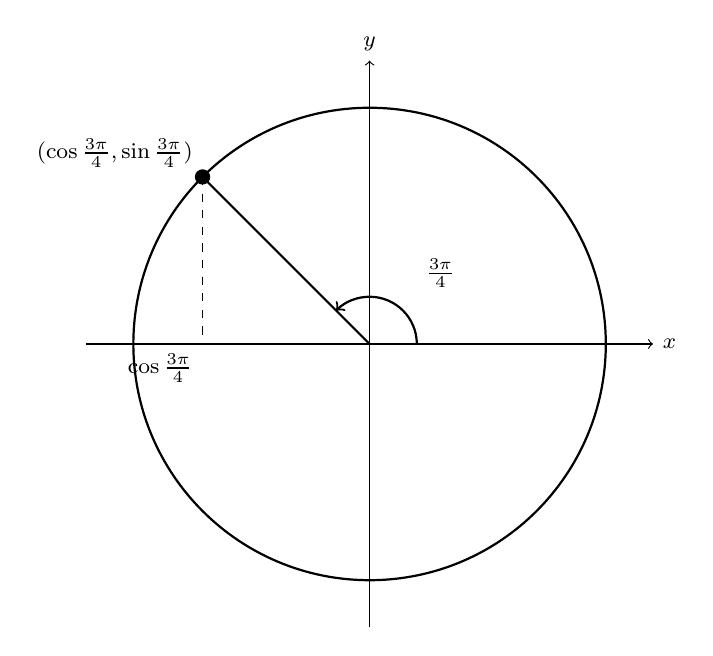
\begin{tikzpicture}[scale=3]
        % Draw the unit circle
        \draw[thick] (0,0) circle(1);

        % Axes
        \draw[->] (-1.2,0) -- (1.2,0) node[right] {\footnotesize $x$};
        \draw[->] (0,-1.2) -- (0,1.2) node[above] {\footnotesize $y$};

        % Angle 3π/4 (135 degrees)
        \draw[thick] (0,0) -- (-0.7071,0.7071);
        \filldraw (-0.7071,0.7071) circle(0.03) node[above left] {\footnotesize $(\cos \frac{3\pi}{4}, \sin \frac{3\pi}{4})$};

        % Draw the cosine value as a horizontal projection
        \draw[dashed] (-0.7071,0.7071) -- (-0.7071,0) node[below left] {\footnotesize $\cos \frac{3\pi}{4}$};

        % Mark the angle
        \draw[thick,->] (0.2,0) arc[start angle=0,end angle=135,radius=0.2];
        \node at (0.3,0.3) {\footnotesize $\frac{3\pi}{4}$};
      \end{tikzpicture}
    \end{center}
    TODO
  \item
    TODO
\end{enumerate}

\subsubsection*{Answer}

\begin{enumerate}[label=(\alph*)]
  \item
    TODO
  \item
    TODO
\end{enumerate}
